\section{Πειράματα κάλυψης χώρου}
\label{section:coverage_tests}

Σκοπός των πειραμάτων κάλυψης χώρου είναι ο υπολογισμός του ποσοστού κάλυψης του χώρου που πραγματοποιείται από το ρομπότ, καθώς και ο χρόνος που απαιτείται για τη διαδικασία αυτή. Θα χρησιμοποιηθούν δύο διαφορετικά περιβάλλοντα, τα οποία έχουν ήδη αναφερθεί προηγουμένως, ο διάδρομος και η αποθήκη, όπου φαίνονται στο \autoref{fig:coverage_worlds} μέσα από τον προσομοιωτή Gazebo. Οι διαστάσεις του πρώτου χώρου είναι $11.65\si{m} \times 2.8\si{m} \times 2.35\si{m}$, ενώ του δεύτερου είναι $19.75\si{m} \times 7.85\si{m} \times 2.4\si{m}$.

\begin{figure}[!ht]
        \begin{subfigure}{0.5\textwidth}
            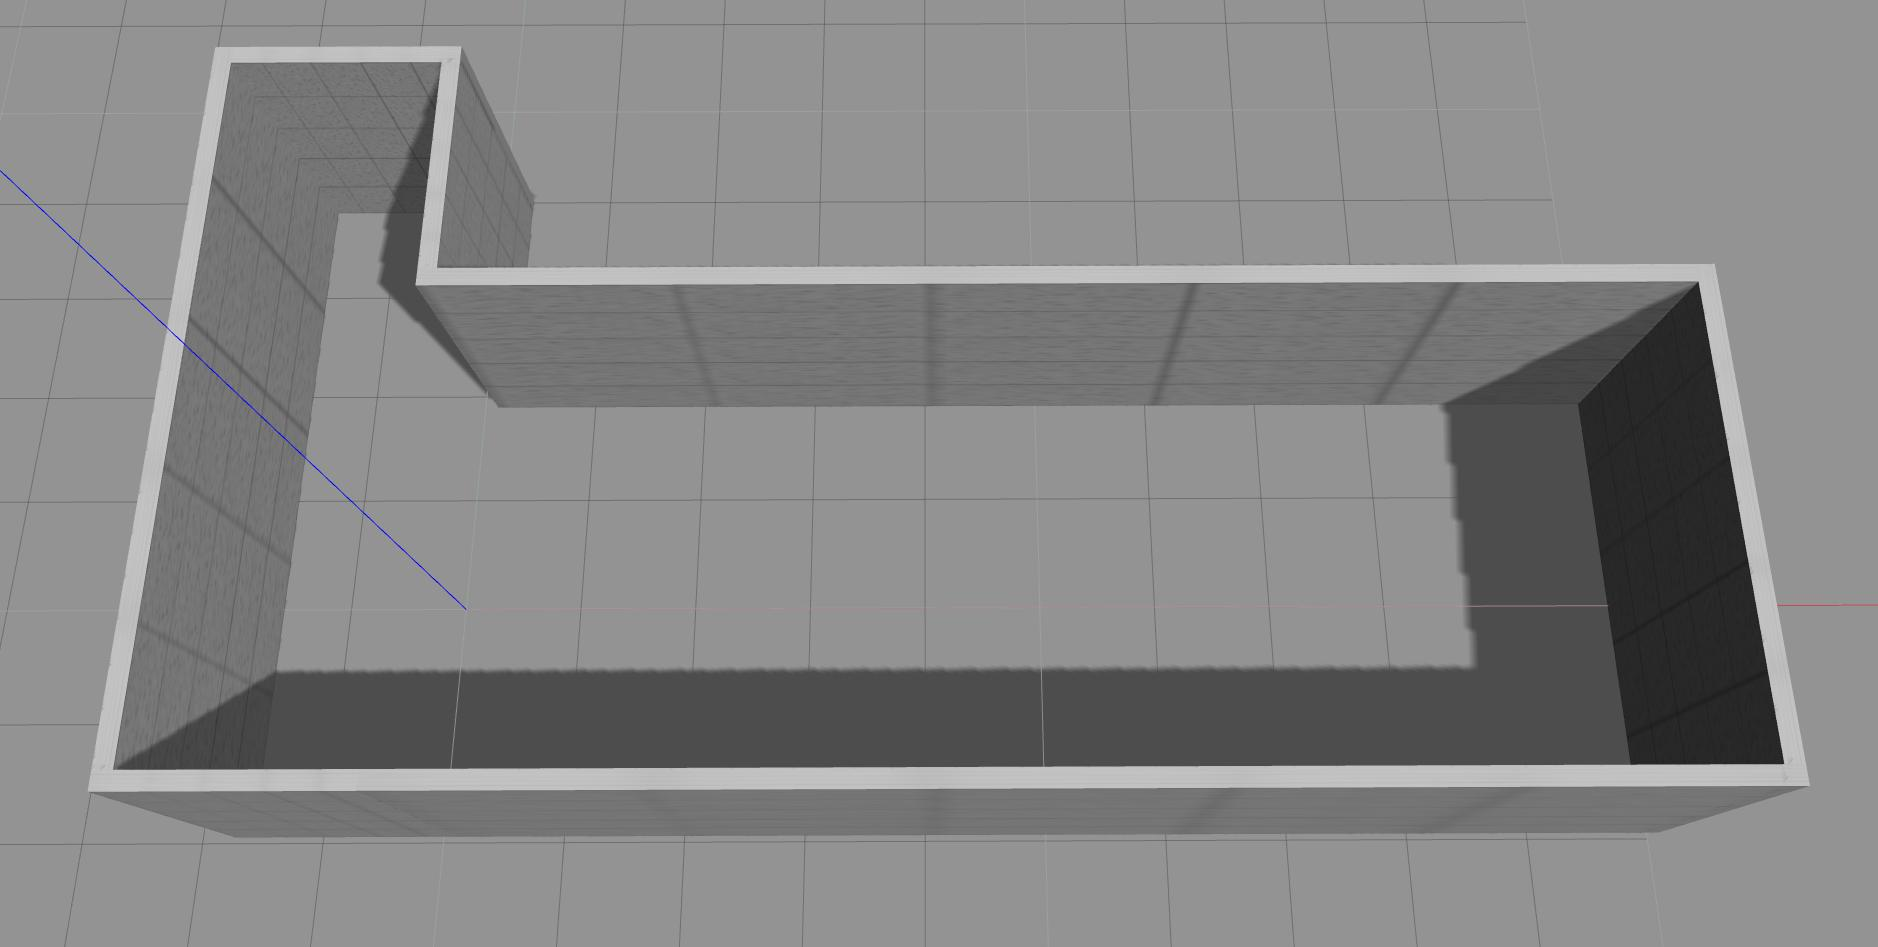
\includegraphics[width=0.9\textwidth]{./images/chapter5/corridor.jpg}
                \caption{Διάδρομος}
             \label{fig:corridor}
        \end{subfigure}
        \begin{subfigure}{0.5\textwidth}
            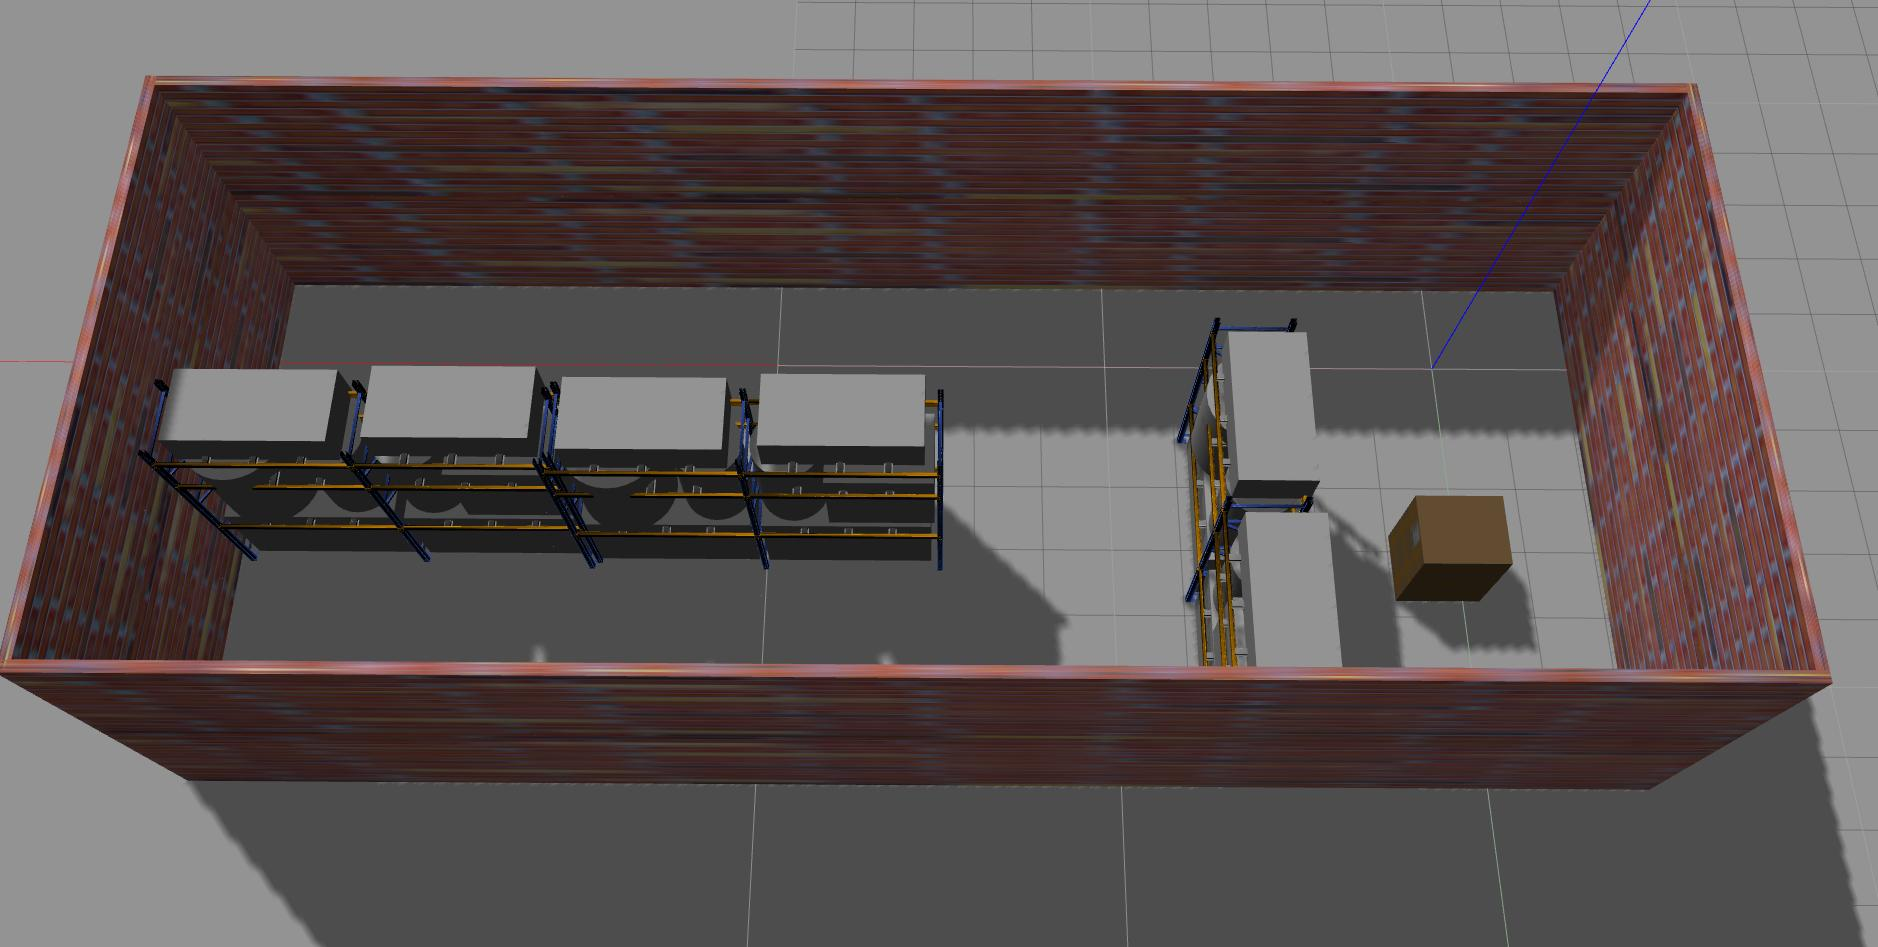
\includegraphics[width=0.9\textwidth]{./images/chapter5/warehouse.jpg}
            \caption{Αποθήκη}
            \label{fig:warehouse}
        \end{subfigure}
        \caption{Περιβάλλοντα που χρησιμοποιήθηκαν στα πειράματα κάλυψης χώρου}
        \label{fig:coverage_worlds}
\end{figure} 

Χρησιμοποιήθηκαν δύο διαφορετικές παραμετροποιήσεις του αισθητήρα RFID, μέσω του οποίου πρέπει να εντοπιστούν όσο το δυνατόν περισσότερα αντικείμενα στον χώρο. Οι τιμές για το ευρύ και στενό οπτικό πεδίο φαίνονται στον \autoref{tab:rfid_configs}.

\begin{table}[H]
    \begin{center}
        \caption{Παράμετροι του αισθητήρα RFID}
        \label{tab:rfid_configs}
        \begin{tabular}{ | c | c | c | c |}
        \hline
        \rowcolor{Gray}
        Τύπος & Οριζόντιο Πεδίο Όρασης & Κάθετο Πεδίο Όρασης & Εύρος\\
        Στενός & \ang{45} & \ang{25} & 1.5 \si{m} \\
        Ευρύς & \ang{80} & \ang{40} & 2.5 \si{m} \\
        \hline
        \end{tabular}
    \end{center}
\end{table}

Για την εύρεση των σημείων τα οποία πρέπει να διασχίσει το ρομπότ για την κάλυψη του χώρου, χρησιμοποιήθηκαν διαφορετικά βήματα δειγματοληψίας, ανάλογα με τον χώρο αλλά και τον αισθητήρα που χρησιμοποιείται σε κάθε περίπτωση. Επίσης, εξετάστηκαν τα διαφορετικά αποτελέσματα ανάλογα με το εάν τα σημεία στον τρισδιάστατο χώρο ενώνονται οριζόντια (slice) ή κάθετα (lift), σύμφωνα με τις μεθόδους που περιγράφονται στο \autoref{section:coverage_impl}. Επίσης, συγκρίνεται η εκτίμηση της κάλυψης του χώρου κατά τη διάρκεια της δημιουργίας του μονοπατιού με την πραγματική κάλυψη που επιτυγχάνεται κατά την κίνηση του ρομπότ στον χώρο. Είναι σημαντικό να επισημάνουμε ότι το σύστημα εντοπισμού θέσης θεωρείται αναγκαίο για να πραγματοποιηθεί μιας ασφαλής και ορθή πλοήγηση του ρομπότ στο χώρο. Η ταχύτητα με την οποία κινήθηκε το drone σε όλες τις περιπτώσεις είναι η χαμηλή, καθώς όπως φαίνεται στο \autoref{section:localization_tests} οδηγεί στο μικρότερο σφάλμα σε όλες τις κινήσεις.

Αρχικά, θα εξεταστούν όλες οι περιπτώσεις για το περιβάλλον του διαδρόμου. Στα διαγράμματα φαίνεται το ποσοστό κάλυψης του χώρου συγκριτικά ως προς τον τρόπο ένωσης των σημείων για ευρύ και στενό οπτικό πεδίο, ενώ στον παρακάτω πίνακα εμφανίζονται συγκεντρωτικά τα αποτελέσματα για κάθε ξεχωριστή περίπτωση.

\begin{figure}[!ht]
    \includegraphics[width=1.0\textwidth]{./images/chapter5/corridor_narrow.png}
    \caption{Ποσοστό κάλυψης συναρτήσει του χρόνου για το περιβάλλον του διαδρόμου με στενό τύπο αισθητήρα}
     \label{fig:corridor_narrow}
\end{figure} 

\begin{figure}[!ht]
    \includegraphics[width=1.0\textwidth]{./images/chapter5/corridor_wide.png}
    \caption{Ποσοστό κάλυψης συναρτήσει του χρόνου για το περιβάλλον του διαδρόμου με ευρύ τύπο αισθητήρα}
     \label{fig:corridor_wide}
\end{figure} 

\begin{table}[!ht]
    \begin{center}
        \caption{Αξιολόγηση κάλυψης χώρου για το περιβάλλον του διάδρομου}
        \label{tab:coverage_corridor}
        \begin{tabular}{ | c | c | c | c | c | c |}
        \hline
        \rowcolor{Gray}
        Τύπος                   & Ένωση     & Βήμα                        & Χρόνος         & Εκτίμηση                 & Πραγματική \\
        \rowcolor{Gray}
                                & σημείων   & δειγματοληψίας              & κάλυψης        & κάλυψης                  & κάλυψη     \\
        \hline
        \multirow{2}{*}{Στενός} & Κάθετη    & \multirow{2}{*}{0.6 \si{m}} & 25.69 \si{min} & \multirow{2}{*}{72.27\%} & 80.76\%    \\
        \cline{2-2}\cline{4-4}\cline{6-6}
                                & Οριζόντια &                             & 43.06 \si{min} &                          & 88.46\%    \\
        \hline
        \multirow{2}{*}{Ευρύς} & Κάθετη     & \multirow{2}{*}{0.6 \si{m}} & 21.70 \si{min} & \multirow{2}{*}{93.30\%} & 88.69\%    \\
        \cline{2-2}\cline{4-4}\cline{6-6}
                               & Οριζόντια  &                             & 18.93 \si{min} &                          & 96.26\%    \\
        \hline
        \end{tabular}
    \end{center}
\end{table}

Παρατηρούμε ότι η χρήση αισθητήρα με ευρύ πεδίο όρασης αποδίδει πολύ καλύτερα συνολικά αποτελέσματα σε συντομότερο χρόνο, όπως ήταν αναμενόμενο. Όταν διαθέτουμε στενό οπτικό πεδίο, το ποσοστό κάλυψης αυξάνεται σχεδόν γραμμικά με το χρόνο, ενώ στην αντίθετη περίπτωση η καμπύλη κάλυψης θυμίζει την λογαριθμική.
    
Αυτό όμως που αξίζει να σημειωθεί είναι η διαφορά που υπάρχει στον τρόπο ένωσης των σημείων ανάλογα με τον τύπο του αισθητήρα. Πιο συγκεκριμένα, για αισθητήρα με στενό FOV η κάθετη ένωση των σημείων οδηγεί σε μικρότερο ποσοστό κάλυψης, χρειάζεται όμως λιγότερο χρόνο για να ολοκληρωθεί. Αντίθετα, στην περίπτωση του ευρυγώνιου αισθητήρα, η οριζόντια ένωση των σημείων οδηγεί σε μεγαλύτερη κάλυψη αλλά και πιο γρήγορη επίτευξη του στόχου. Η διαφορά που παρατηρείται ανάμεσα στην εκτίμηση της κάλυψης και την πραγματική, οφείλεται στην κίνηση του drone μέσα στον χώρο που οδηγεί είτε σε σημεία τα οποία δεν είχαν υπολογιστεί εκ των προτέρων, είτε σε αστοχία ορισμένων αρχικών στόχων.

Παρακάτω παρουσιάζονται τα αντίστοιχα αποτελέσματα για το περιβάλλον της αποθήκης.

\begin{figure}[!ht]
    \includegraphics[width=1.0\textwidth]{./images/chapter5/warehouse_narrow.png}
    \caption{Ποσοστό κάλυψης συναρτήσει του χρόνου για το περιβάλλον της αποθήκης με στενό τύπο αισθητήρα}
     \label{fig:warehouse_narrow}
\end{figure} 

\begin{figure}[!ht]
    \includegraphics[width=1.0\textwidth]{./images/chapter5/warehouse_wide.png}
    \caption{Ποσοστό κάλυψης συναρτήσει του χρόνου για το περιβάλλον της αποθήκης με ευρύ τύπο αισθητήρα}
     \label{fig:warehouse_wide}
\end{figure} 

\begin{table}[H]
    \begin{center}
        \caption{Αξιολόγηση κάλυψης χώρου για το περιβάλλον της αποθήκης}
        \label{tab:coverage_warehouse}
        \begin{tabular}{ | c | c | c | c | c | c |}
        \hline
        \rowcolor{Gray}
        Τύπος                   & Ένωση     & Βήμα                        & Χρόνος         & Εκτίμηση                 & Πραγματική \\
        \rowcolor{Gray}
                                & σημείων   & δειγματοληψίας              & κάλυψης        & Κάλυψης                  & Κάλυψη     \\
        \hline
        \multirow{2}{*}{Στενός} & Κάθετη    & \multirow{2}{*}{0.8 \si{m}} & 40.40 \si{min} & \multirow{2}{*}{50.18\%} & 65.43\%    \\
        \cline{2-2}\cline{4-4}\cline{6-6}
                                & Οριζόντια &                             & 76.52 \si{min} &                          & 72.49\%    \\
        \hline
        \multirow{2}{*}{Ευρύς} & Κάθετη     & \multirow{2}{*}{0.9 \si{m}} & 37.18 \si{min} & \multirow{2}{*}{62.33\%} & 84.12\%    \\
        \cline{2-2}\cline{4-4}\cline{6-6}
                               & Οριζόντια  &                             & 46.59 \si{min} &                          & 84.88\%    \\
        \hline
        \end{tabular}
    \end{center}
\end{table}

Στην περίπτωση αυτή χρησιμοποιήθηκε μεγαλύτερο βήμα δειγματοληψίας, καθώς πρόκειται για έναν μεγαλύτερο σε έκταση χώρο. Παρατηρούμε πάλι την ίδια συμπεριφορά με πριν στις καμπύλες κάλυψης και των δύο τύπων αισθητήρα. Ανεξαρτήτως στενού ή ευρύ οπτικού πεδίου, η ένωση των σημείων με κάθετο τρόπο οδηγεί σε συντομότερη ολοκλήρωση της διαδικασίας κάλυψης. Όμως, το τελικό ποσοστό είναι μεγαλύτερο όταν χρησιμοποιείται η οριζόντια ένωση των σημείων. Πιο αναλυτικά, όταν διαθέτουμε στενό FOV η χρονική διαφορά είναι μεγάλη και αυτό οφείλεται σε όλα τα διαφορετικά ύψη τα οποία πρέπει να βρεθεί το ρομπότ, ώστε να καλύψει ολόκληρο το χώρο. Σε όλες τις περιπτώσεις, είναι χαρακτηριστική η διαφορά της κάλυψης από την εκτίμηση κάλυψης, κάτι που δημιουργείται λόγω της μεγαλύτερης σε διάρκεια κίνησης του ρομπότ στον χώρο.

Στην αποθήκη, καθώς πρόκειται για ένα πιο περίπλοκο περιβάλλον, το συνολικό ποσοστό κάλυψης είναι μικρότερο από ότι θα ήταν το επιθυμητό για την πλήρη κάλυψη. Αυτό όμως οφείλεται και στις ιδιαιτερότητες του χάρτη, με την ύπαρξη σημείων που είναι αδύνατον να ανιχνευτούν από το ρομπότ και δεν αφαιρέθηκαν με την επεξεργασία των σημείων κατά τον υπολογισμό του όγκου που περιγράφηκε προηγουμένως.